\documentclass{handout}

% \SetInstructor{Lt Col James Phillips}
\SetCourseTitle{ECE231: Electrical Circuits and Systems I}
\SetSemester{Fall 2016}
\SetHandoutTitle{Lecture 35: Filters III -- Band Pass and Band Reject Filters}

%\SetDueDate{1 Jan 2016}
%\ShowAllBlanks

\showsoln \setsolncolor{red}

\begin{document}
\maketitle

\textbf{OBJECTIVES:}
\begin{enumerate}
\item Understand the operation of Band Pass Filters (BPF) and Band Reject Filters (BRF)
\item Be able to design BPF and BRF using LPF and HPF as building blocks
\end{enumerate}

\textbf{READING}
\begin{description}
\item [Required]:
Filters Handout (Available on Sharepoint), pgs 35--38
\end{description}

\section{Introduction}
Last lesson we talked about Low Pass and High Pass Filters; today we are going to look at how we can use these simple filters as building blocks to build two new types of filter: the Band Pass Filter (BPF) and the Band Reject Filter (BRF).  It should be easy to figure out what these filters do from their name.  A {\em Band Pass} Filter passes a signal when the the frequency is in a passband defined by two frequencies, $\omega_{c1}$ and $\omega_{c2}$.  A {\em Band Reject} Filter rejects signals whose frequency are {\em in band}.

\section{Block Diagrams of BPF and BRF}
Before we talk about the actual design of these filters, lets step back and look at them as block diagrams using LPFs and HPFs as our building blocks.

\subsection{BPF}
Let's start by looking at a graph of an {\em ideal} Band Pass Filter Transfer function.

\soln{1.5in}{
This figure is hidden is student copy
\begin{figure} [h!]
\centering
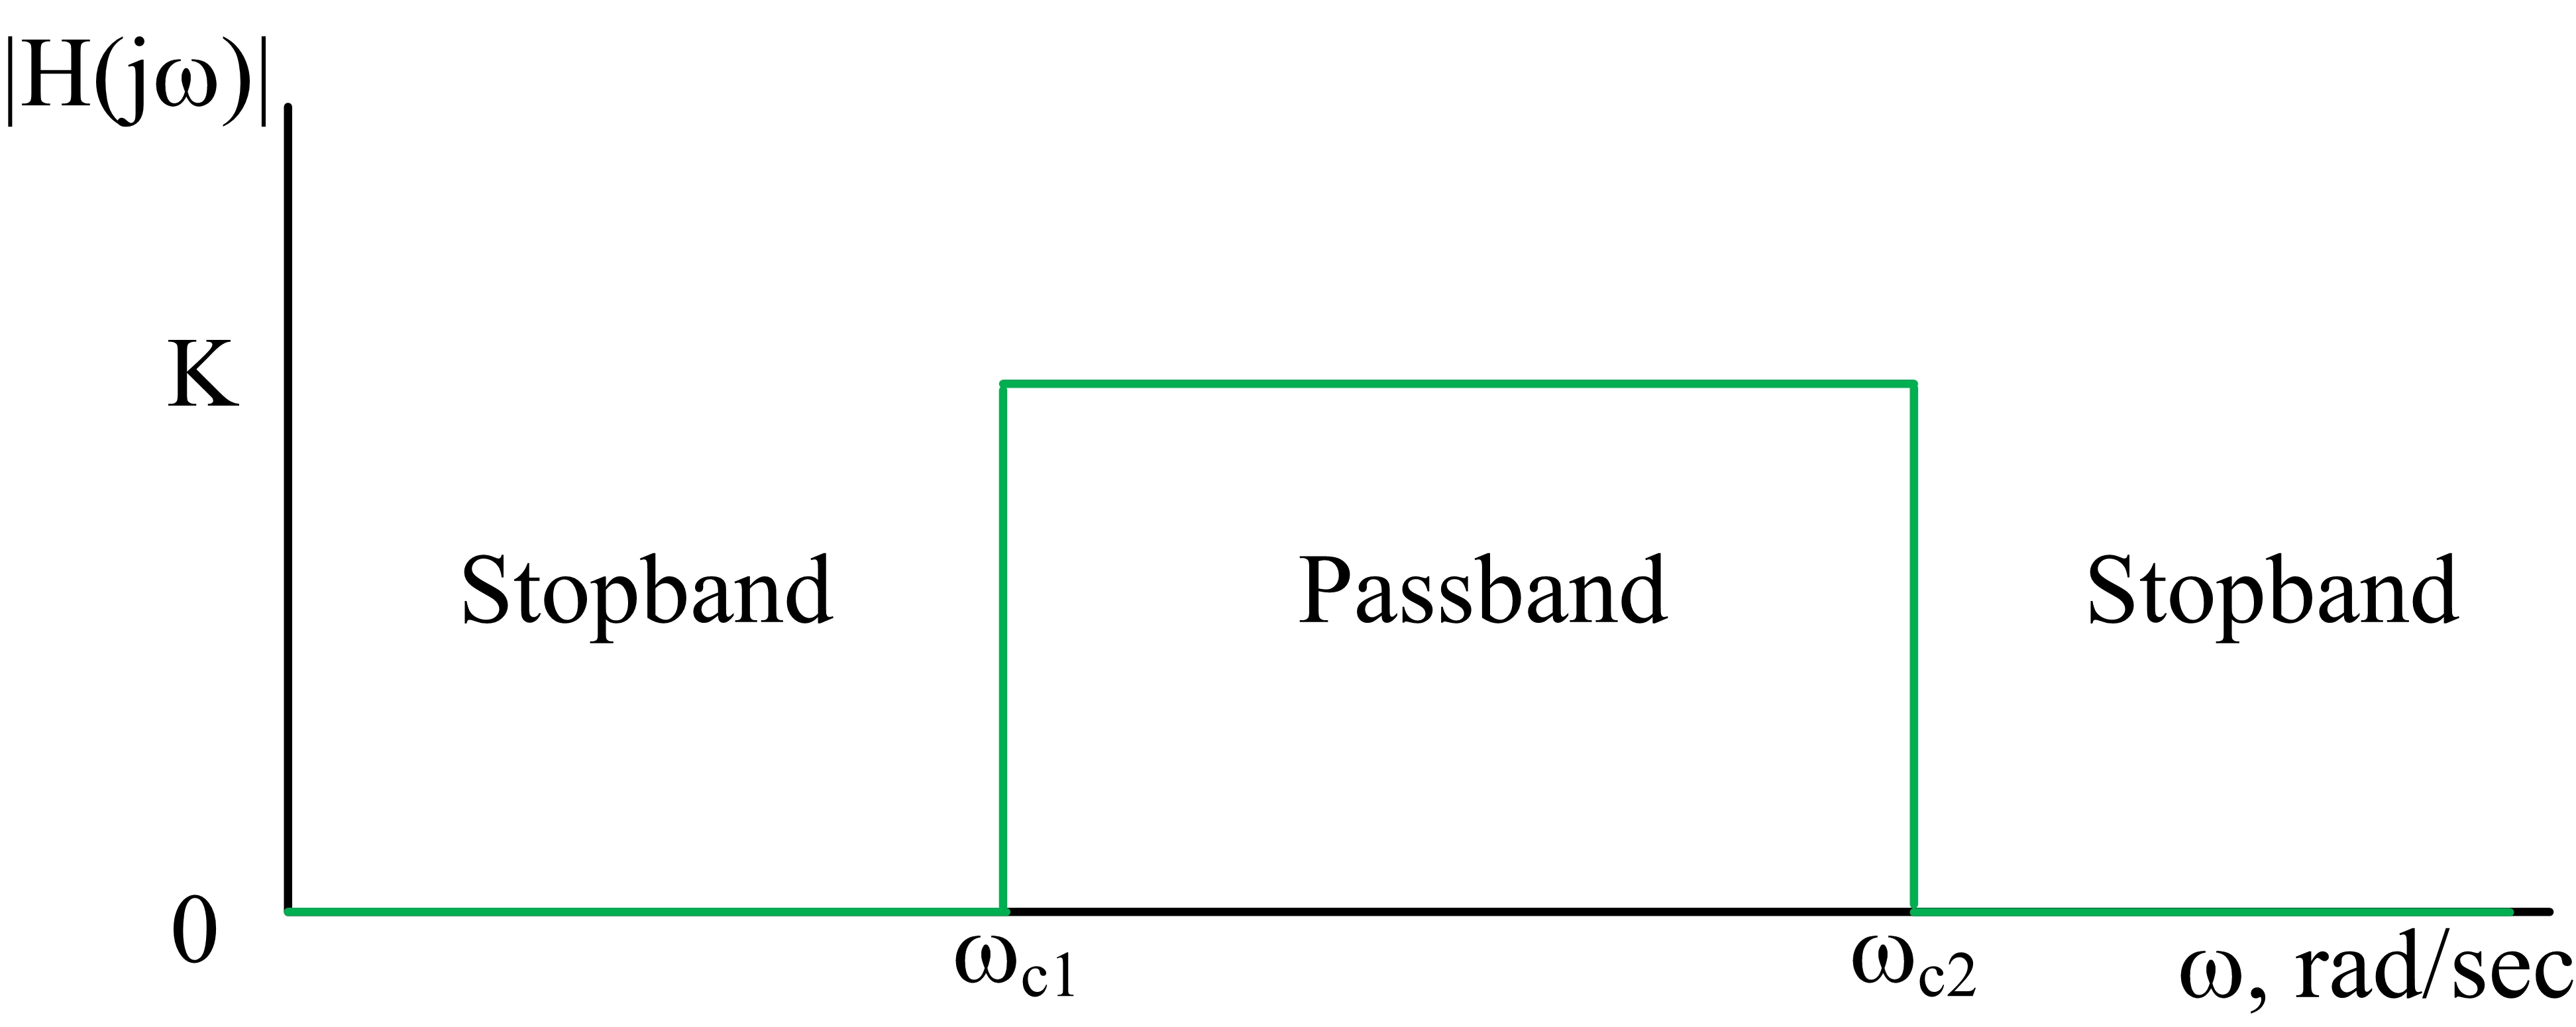
\includegraphics[width=0.8\textwidth]{BandpassTransferFunction.jpg}
\end{figure}
}

If we want to build this filter with combination of a LPF and a HPF, we can {\em cascade} the transfer functions to arrive at

\soln{1.5in}{
This figure is hidden is student copy
\begin{figure} [h!]
\centering
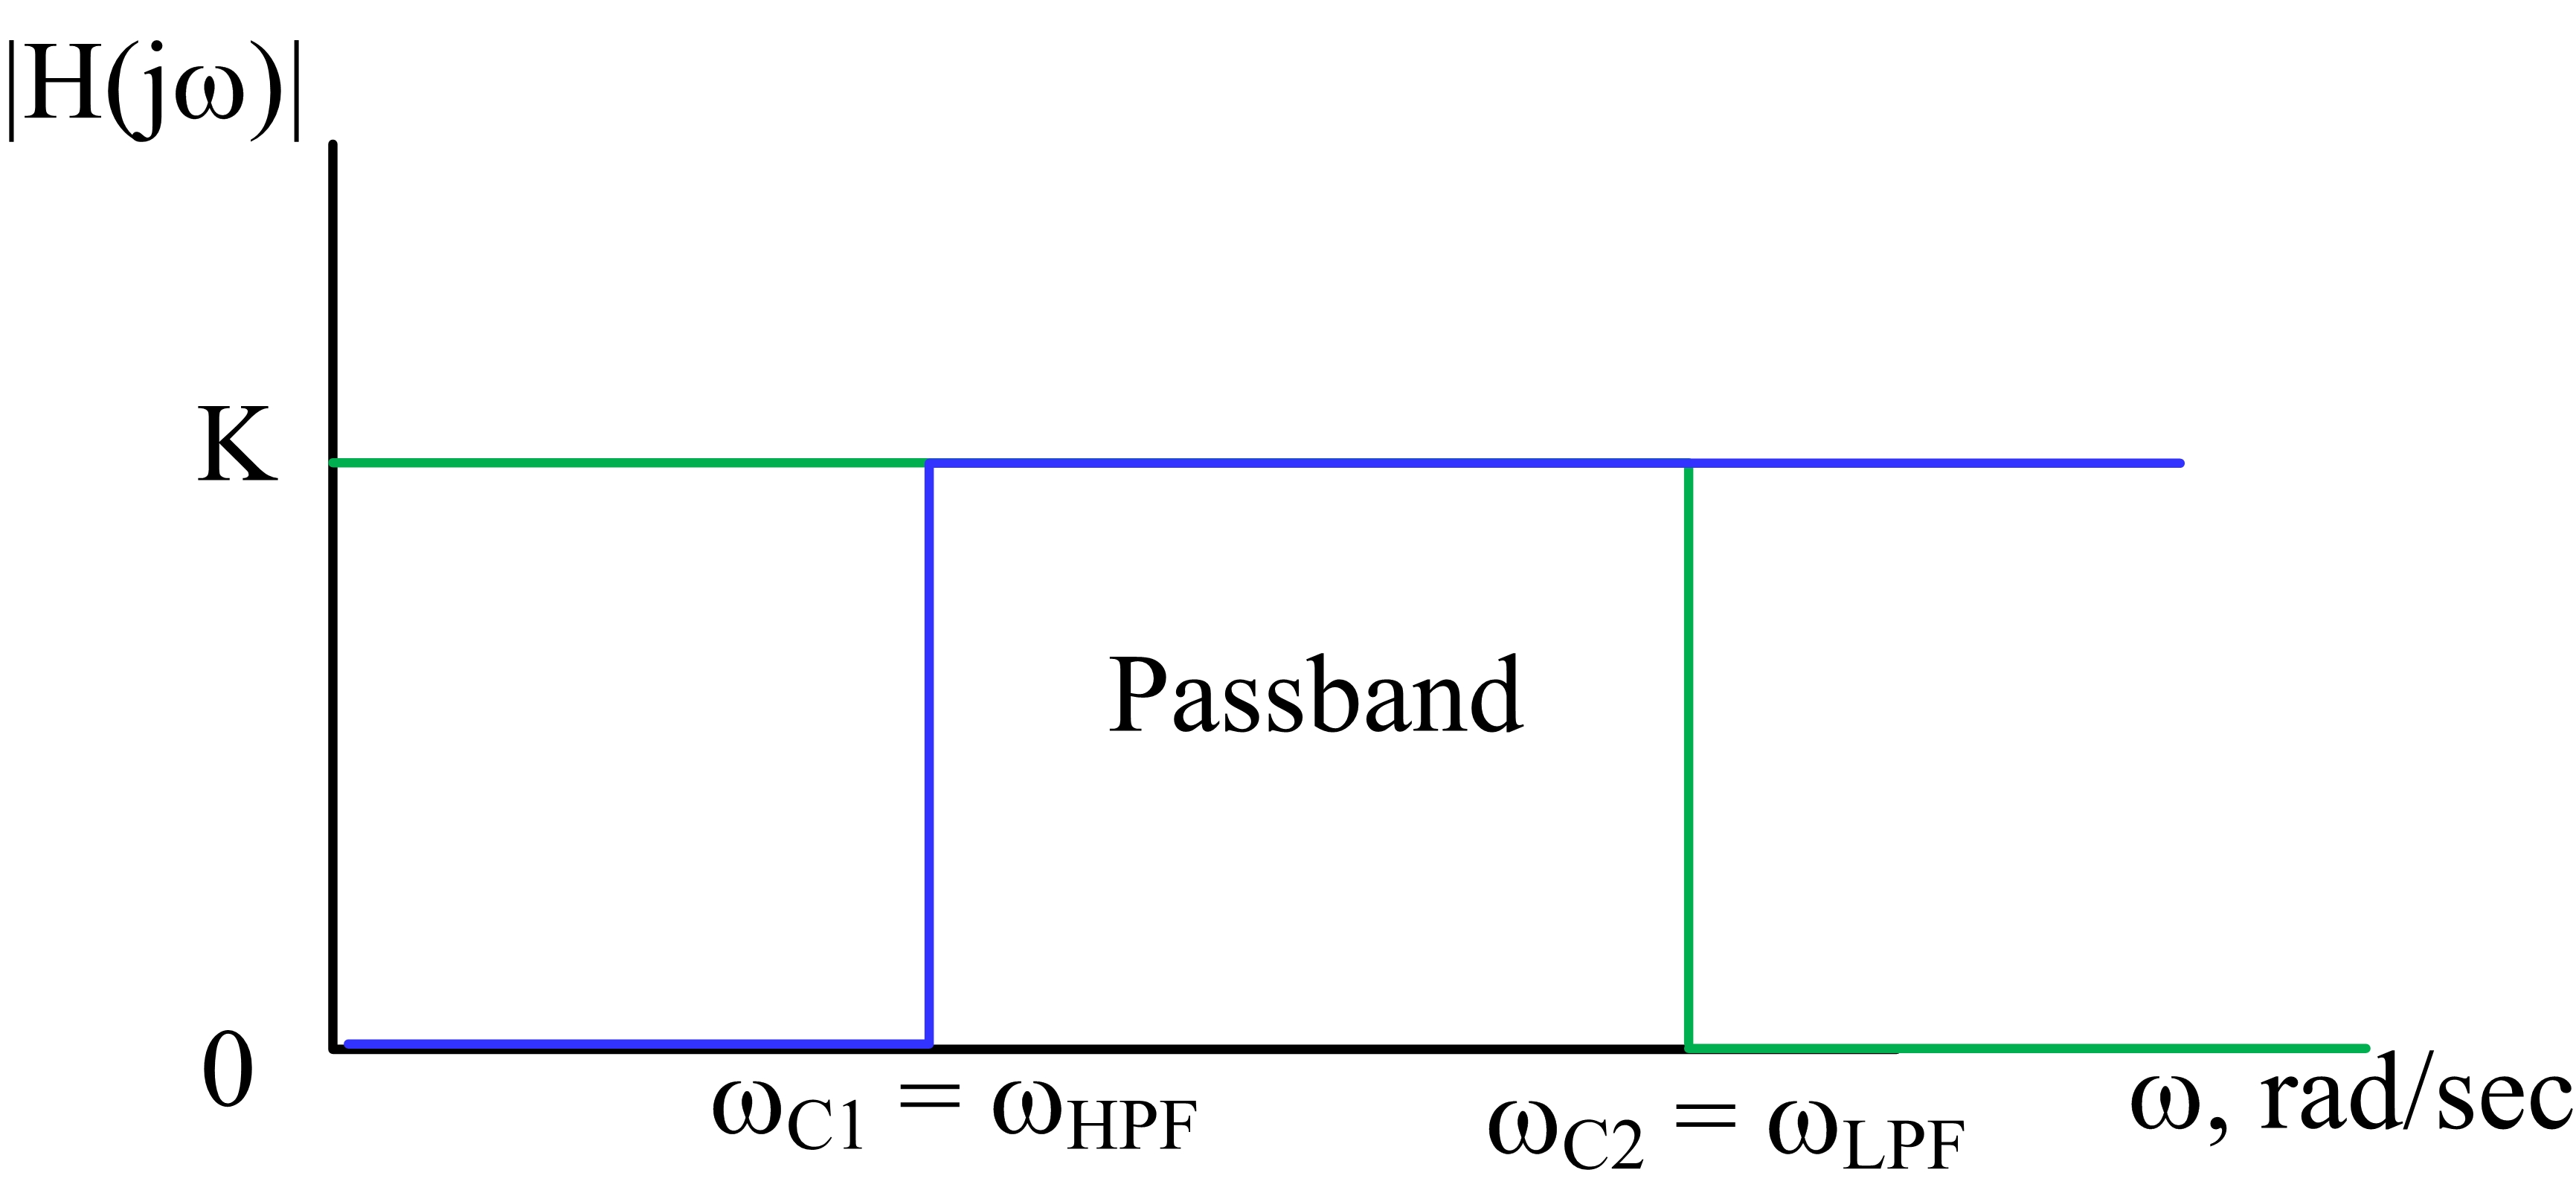
\includegraphics[width=0.8\textwidth]{BandpassTransferFunction2.jpg}
\end{figure}
}

A block diagram of this filter would look like:

\soln{1.5in}{
This figure is hidden is student copy
\begin{figure} [h!]
\centering
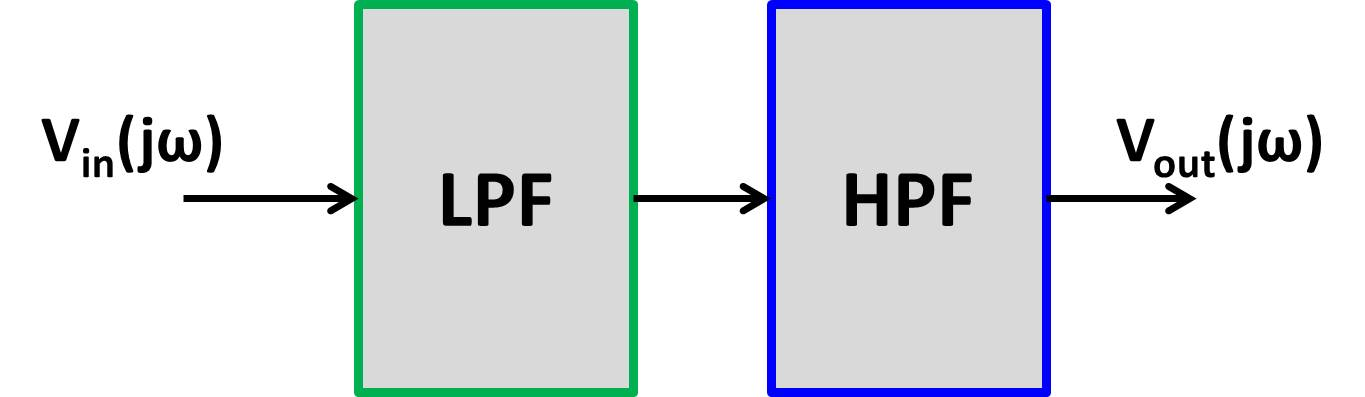
\includegraphics[width=0.5\textwidth]{BPFBlockDiagram.jpg}
\end{figure}

Note: The order of the filters is not important
}

A very important thing to remember is when designing a BPF, the cut-off for the HPF must be {\em smaller} than the cut-off of the LPF.  \textbf{What happens if the HPF cut-off is {\em larger} than the LPF cut-off?}  \soln{0.5in}{You have designed a NO-PASS filter!}

\subsection{BRF}
Let's now look at a graph of an {\em ideal} Band Reject Filter Transfer function.

\soln{1.5in}{
This figure is hidden is student copy
\begin{figure} [h!]
\centering
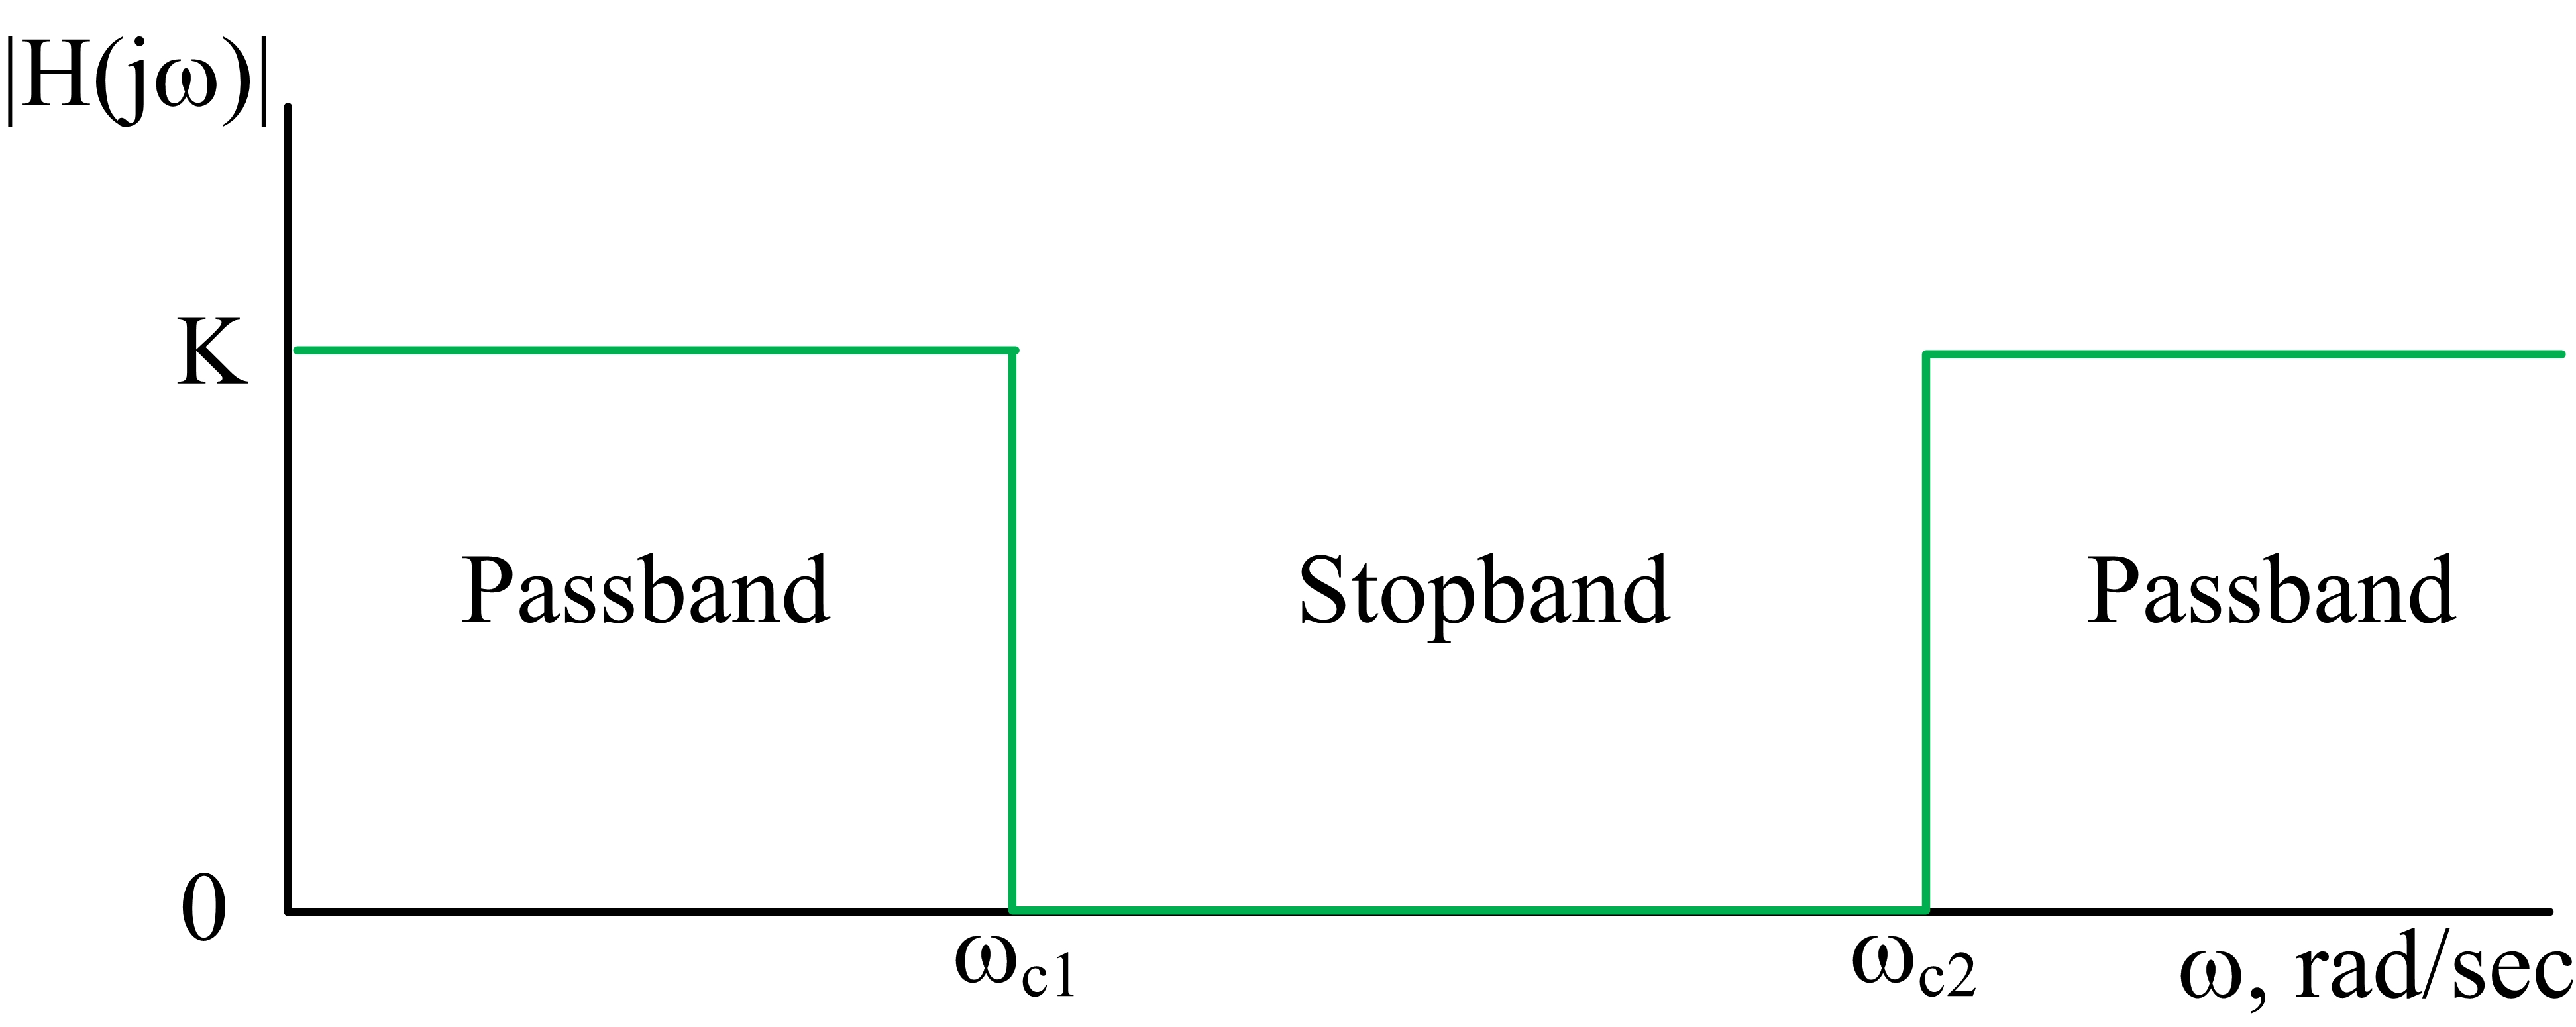
\includegraphics[width=0.8\textwidth]{BRFTransferFunction.jpg}
\end{figure}
}

I hope at this point it is obvious we can build this by {\em connecting} a LPF and a HPF; what is probably not obviouse is how we connect them.  \textbf{To build a BRF, you cannot cascade a LPF and a HPF!}

To build a Band Reject Filter, we will connect a LPF and a HPF using a summer:

\soln{1.5in}{
This figure is hidden is student copy
\begin{figure} [h!]
\centering
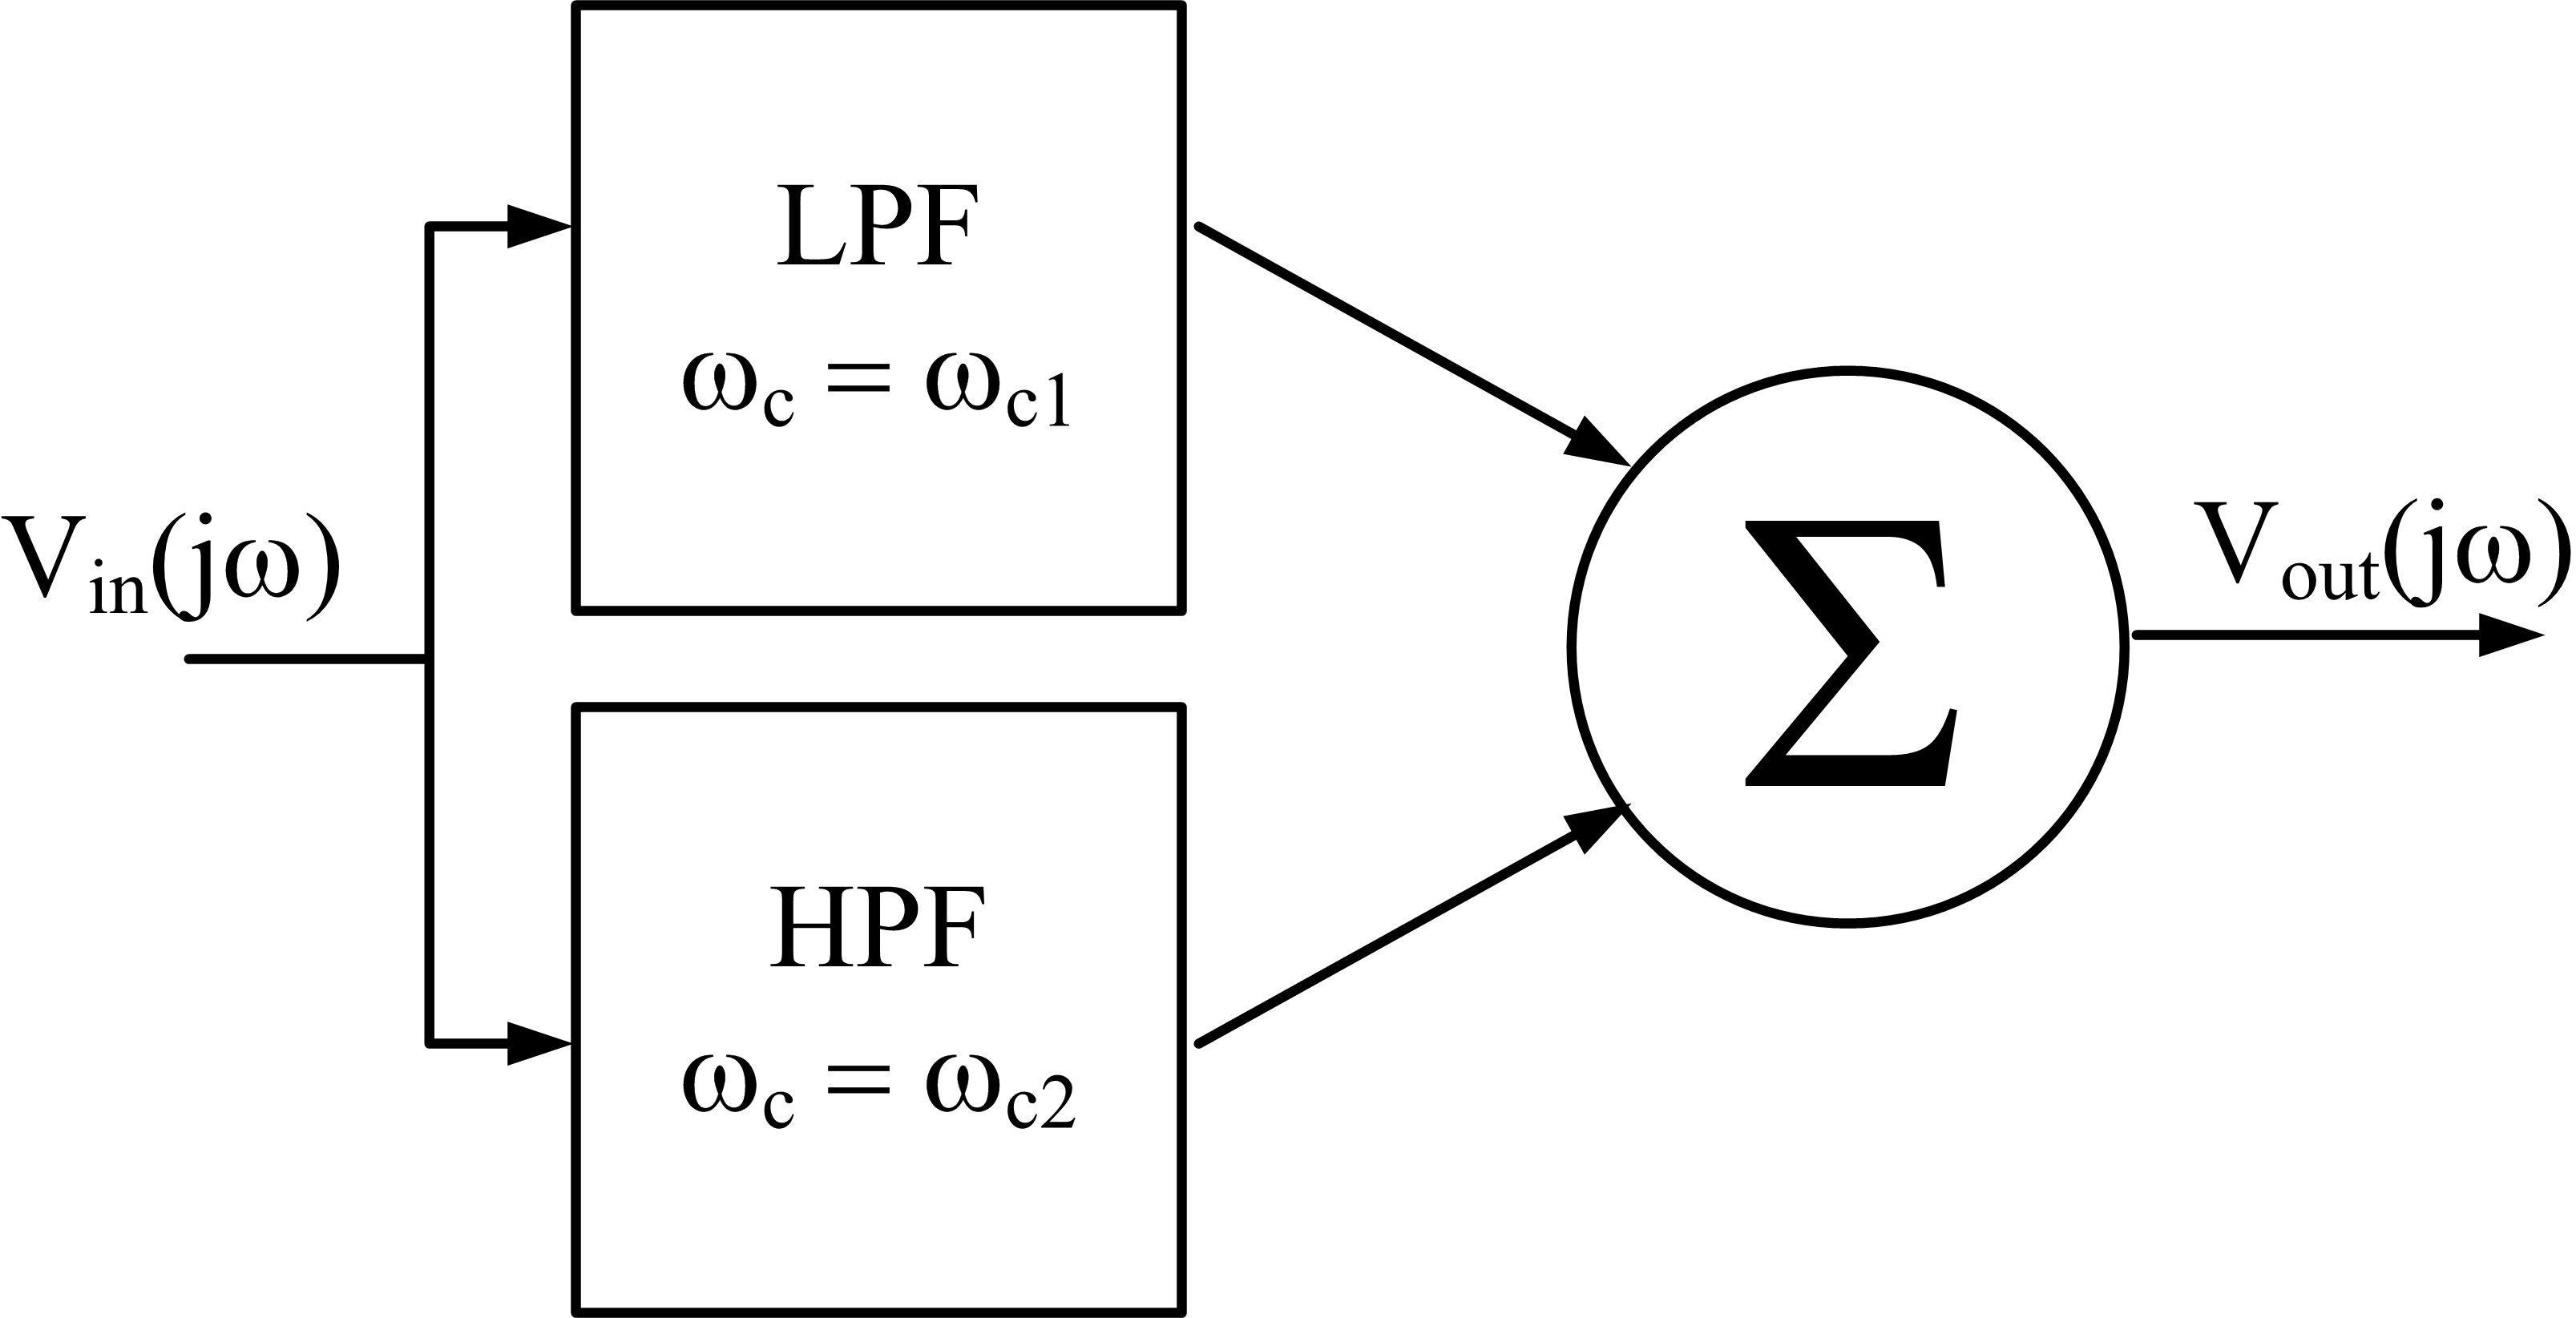
\includegraphics[width=0.5\textwidth]{BRFBlockDiagram.jpg}
\end{figure}
}

A very important thing to remember is when designing a BRF, the cut-off for the HPF must be {\em larger} than the cut-off of the LPF.  \textbf{What happens if the HPF cut-off is {\em smaller} than the LPF cut-off?}  \soln{0.5in}{You have designed an ALL-PASS filter!}

\newpage
\clearpage
\pagebreak

\section{Designing Real Band Pass Filters}
Let's look at the example from section 4.1 of the reading.

\textbf{Example 1}--Let's design a BPF with $\omega_{c1}=500\frac{rad}{s}$ and $\omega_{c2}=10,000\frac{rad}{s}$:

\soln{4in}{
First we will design a LPF with a cut-off of $\omega_{c2}=10,000\frac{rad}{s}$.  Recalling our standard form for a LPF transfer function we can write:
\[
H_{LPF}(j\omega) = \frac{10,000}{j\omega +10,000}
\]
Next we deisgn a HPF with a cut-off of $\omega_{c1}=500\frac{rad}{s}$.   Recalling our standard form for a HPF transfer function we can write:
\[
H_{HPF}(j\omega) = \frac{j\omega}{j\omega +500}
\]
Finally we cacade the two transfer functions to arrive at:
\[
H_{BPF}(j\omega) = \frac{10,000}{j\omega +10,000}\frac{j\omega}{j\omega +500}=\frac{j10,000\omega}{(j\omega)^2+j10,500\omega +5,000,000}
\]

We can plot the phase and magnitude of this transfer function:
\begin{figure} [h!]
\centering
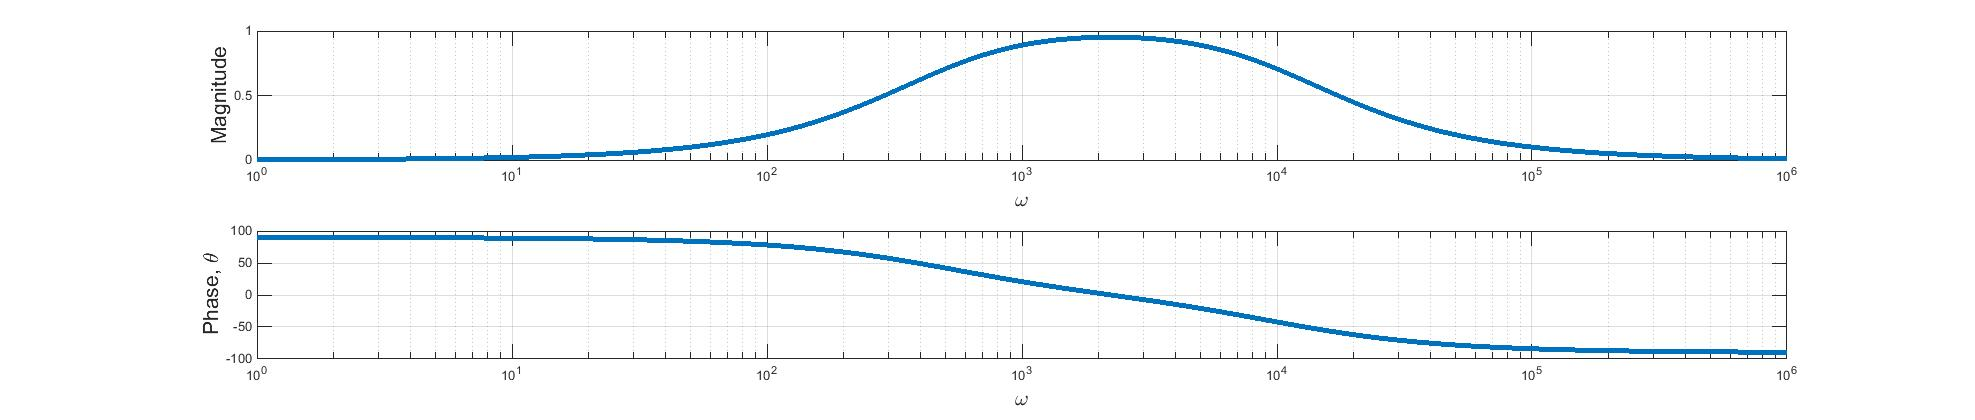
\includegraphics[width=1\textwidth]{Example1soln.jpg}
\end{figure}

The magnitude response is what we would expect for a BPF and the phase response is zero at the center of the passband.
}

\newpage
\clearpage
\pagebreak

\textbf{How would we actually build the filter from our example above?}


What if we simply cascaded a LPF and a HPF as shown below?
\begin{figure} [h!]
\centering
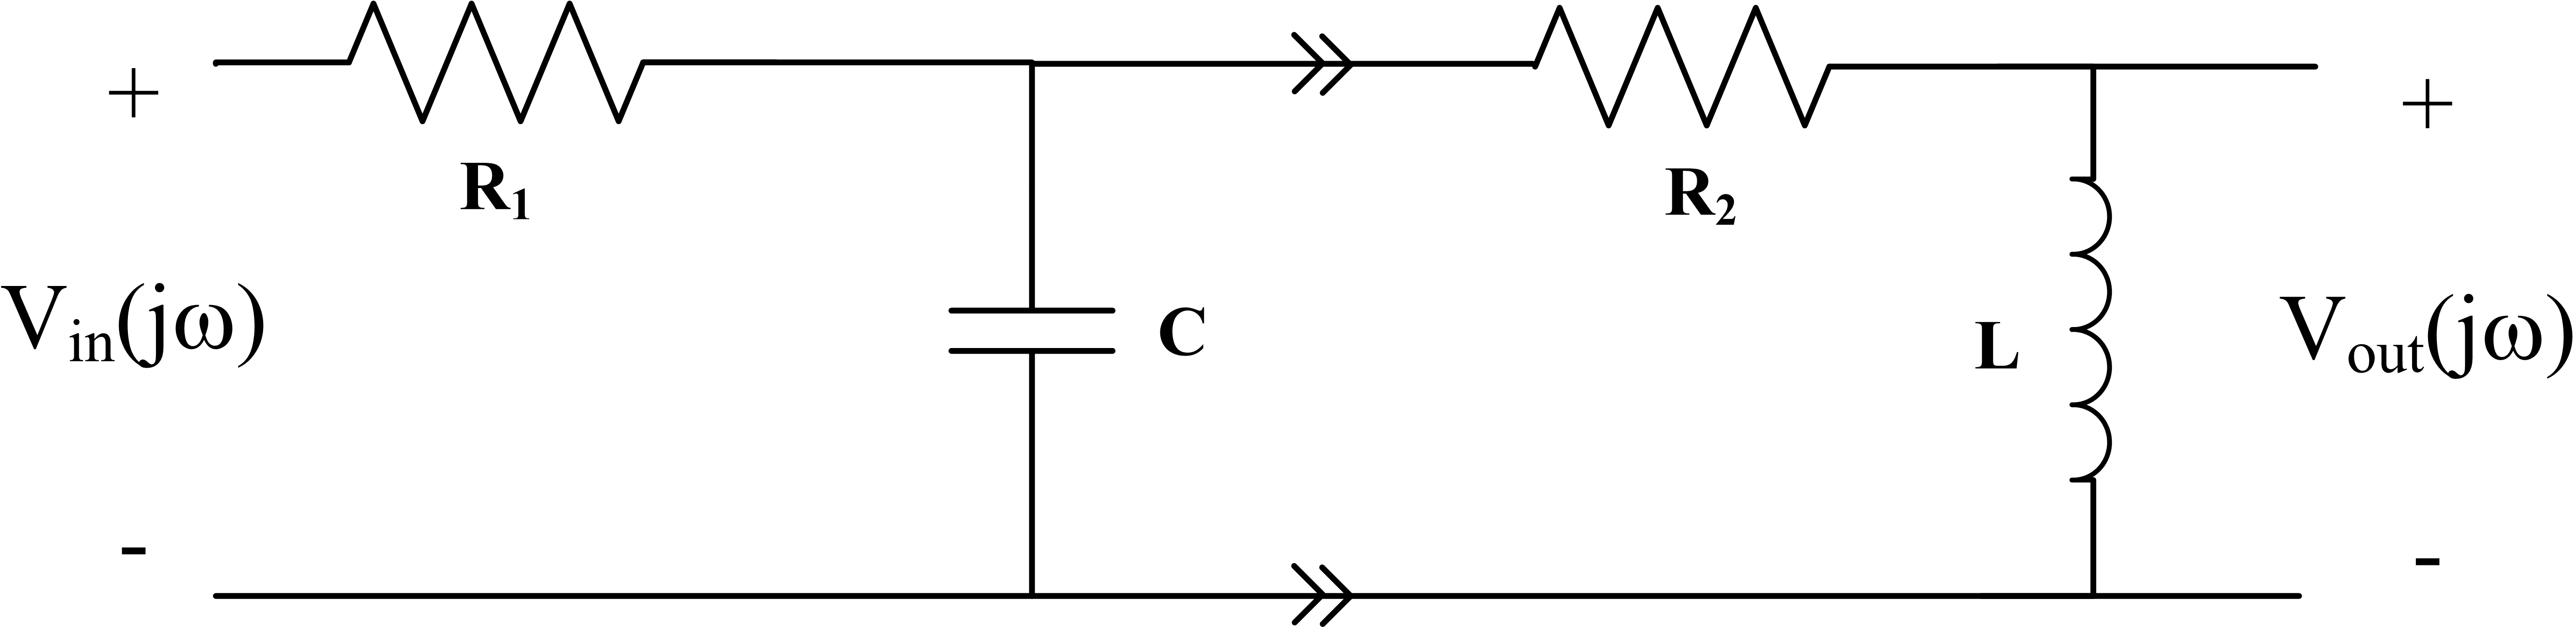
\includegraphics[width=0.7\textwidth]{BPF1.jpg}
\end{figure}

\soln{8in}{
We need to find values for the resistors, capacitor and inductor.  We know:
\[
\frac{1}{R_1C}=10,000\frac{rad}{s}
\]
\[
\frac{R_2}{L} = 500\frac{rad}{s}
\]

To satisfy the above requirements, we can use:
\[
R_1=1\ k\Omega
\]
\[
C=0.1\ \mu F
\]
\[
R_2 = 500\Omega
\]
\[
L=1H
\]

If we write Node Voltage equations for this circuit we get:
\[
\frac{V_A - V_{IN}}{R_1} + V_Aj\omega C + \frac{V_A - V_{OUT}}{R_2} = 0
\]
\[
\frac{V_{OUT} - V_A}{R_2} + \frac{V_{OUT}}{j\omega L}  = 0
\]

We can write the system of equations in matrix form:
\[
\left[\begin{array}{cc}
\frac{1}{R_1}+j\omega C + \frac{1}{R_2} & -\frac{1}{R_2} \\
-\frac{1}{R_2} & \frac{1}{R_2}+\frac{1}{j\omega L}
\end{array}\right]\left[\begin{array}{c}
V_A \\
V_{OUT}
\end{array}\right] = \left[\begin{array}{c}
\frac{V_{IN}}{R_1} \\
0
\end{array}\right]
\]

You can know use Matlab's symnbolic toolbox to get the transfer function, Matlab will output (the output will not look this clean):
\[
V_{out}=\frac{10,000V_{in}\omega}{j\omega^2+10,500\omega-j15,000,000}
\]
Which we can divide out the $V_{in}$ and manipulate into standard form of a transfer function to arrive at:
\[
H(j\omega)=\frac{j10,000\omega}{(j\omega)^2+j10,500\omega+15,000,000}
\]

This is very similar to what is in the reading, however, itis not exact; it also does not match what we expect from cascading these filters.  The root cause of both of these issues is stage loading!
}


\newpage
\clearpage
\pagebreak

To avoid stage loading we insert a buffer between the two stages as shown below:

\soln{2in}{
This figure is hidden is student copy
\begin{figure} [h!]
\centering
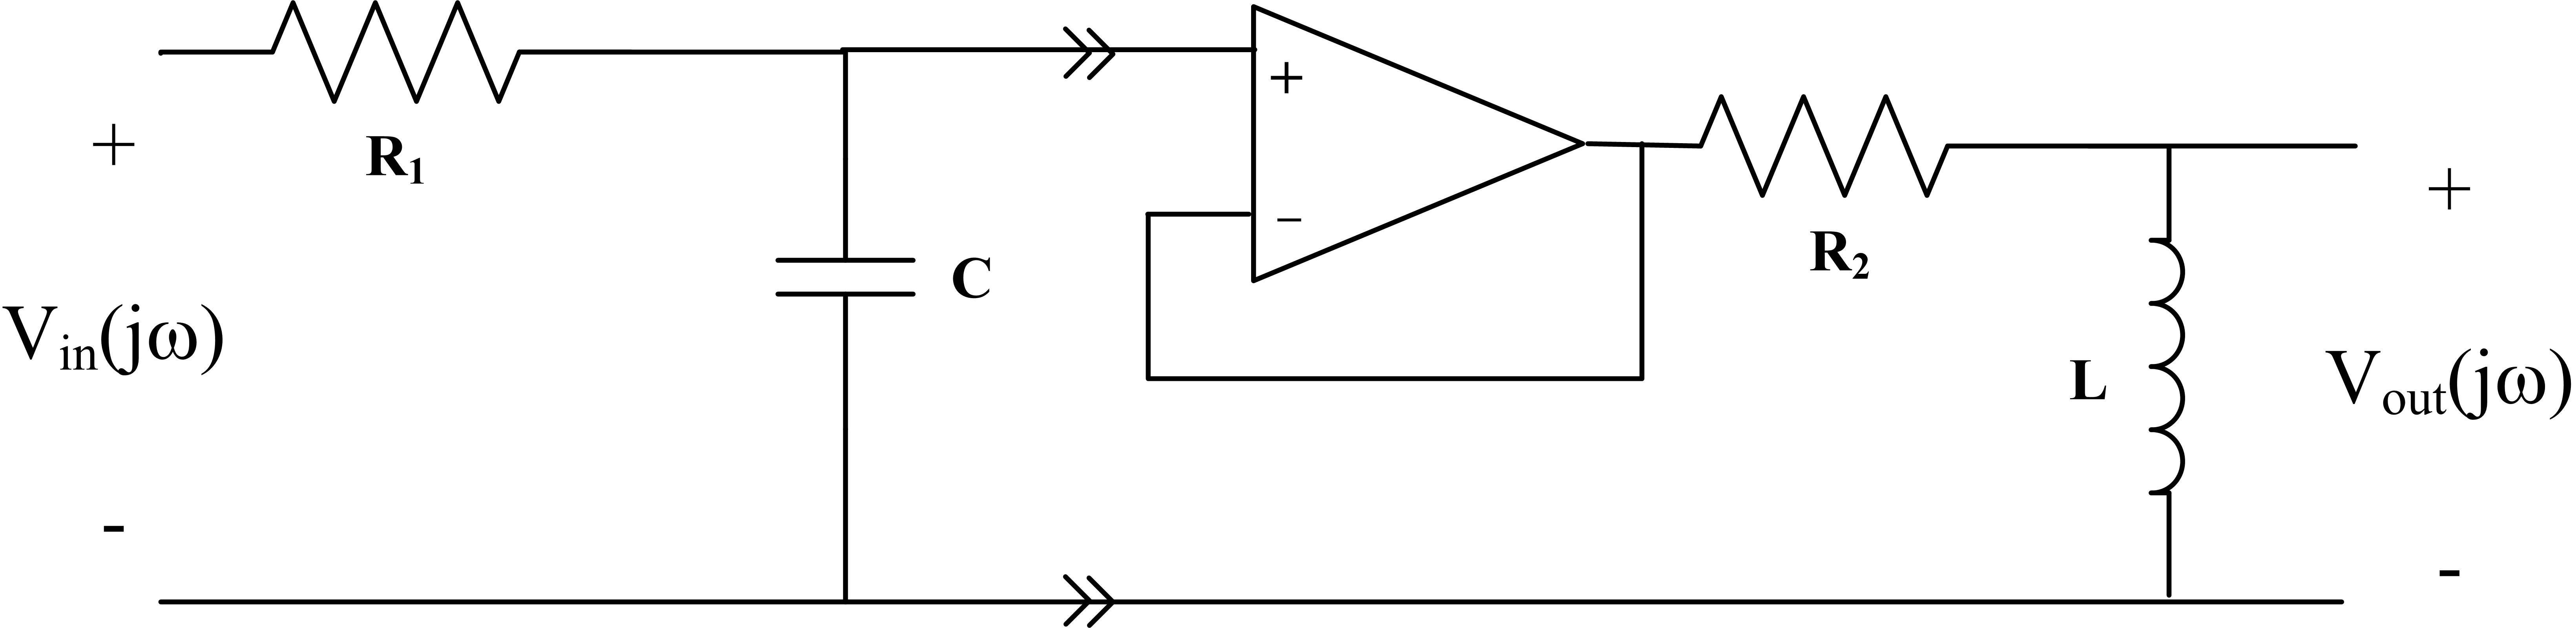
\includegraphics[width=0.9\textwidth]{BPF2.jpg}
\end{figure}

The transfer function for this circuit is:
\[
H(j\omega) =\frac{j10,000\omega}{(j\omega)^2+j10,500\omega +5,000,000}
\]
}

If we need an amplification stage ($K>1$), we can replace the buffer with a {\em non-inverting amplifier} as shown below:

\soln{2in}{
This figure is hidden is student copy
\begin{figure} [h!]
\centering
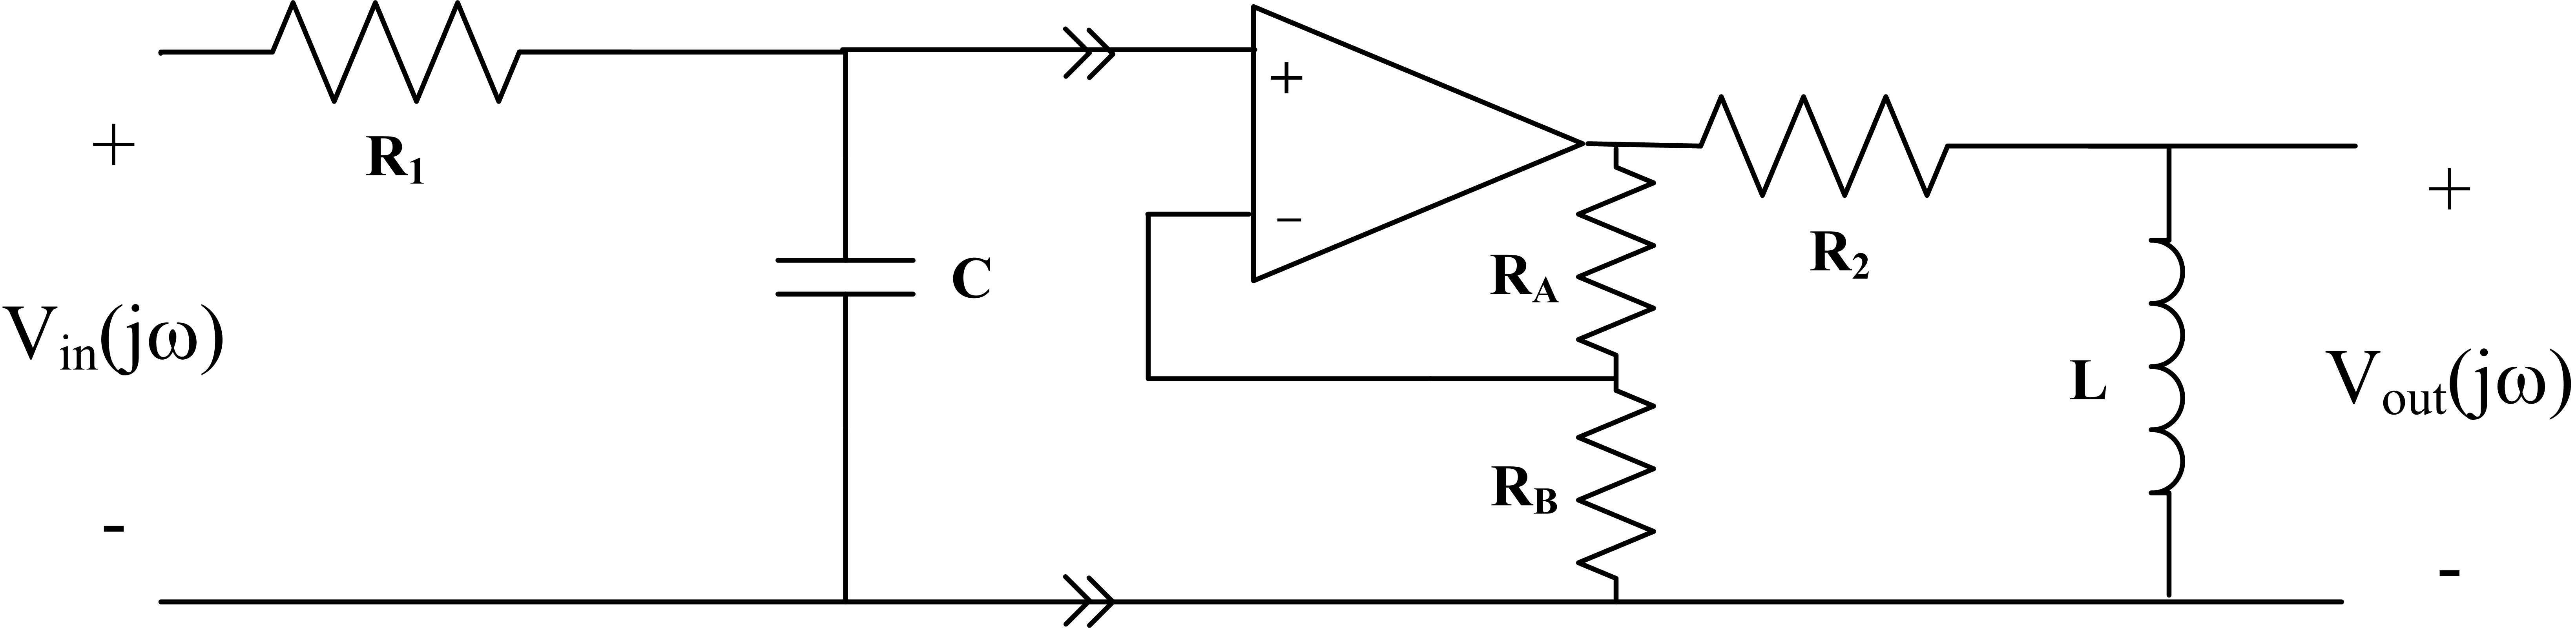
\includegraphics[width=0.9\textwidth]{BPF3.jpg}
\end{figure}
The transfer function for this circuit is:
\[
H(j\omega) =\left[\frac{R_A+R_B}{R_B}\right]\left[\frac{j10,000\omega}{(j\omega)^2+j10,500\omega +5,000,000}\right]
\]
}

\newpage
\clearpage
\pagebreak

\section{Designing Real Band Reject Filters}
Let's look at the example from section 4.2 of the reading.

\textbf{Example 1}--Let's design a BRF with $\omega_{c1}=500\frac{rad}{s}$ and $\omega_{c2}=10,000\frac{rad}{s}$:

\soln{4in}{
First we will design a LPF with a cut-off of $\omega_{c1}=500\frac{rad}{s}$.  Recalling our standard form for a LPF transfer function we can write:
\[
H_{LPF}(j\omega) = \frac{500}{j\omega +500}
\]
Next we deisgn a HPF with a cut-off of $\omega_{c2}=10,000\frac{rad}{s}$.   Recalling our standard form for a HPF transfer function we can write:
\[
H_{HPF}(j\omega) = \frac{j\omega}{j\omega +10,000}
\]
Finally we \textbf{SUM} the two transfer functions to arrive at:
\[
H_{BRF}(j\omega) = \frac{500}{j\omega +500}+\frac{j\omega}{j\omega +10,000}
\]

We can plot the phase and magnitude of this transfer function:
\begin{figure} [h!]
\centering
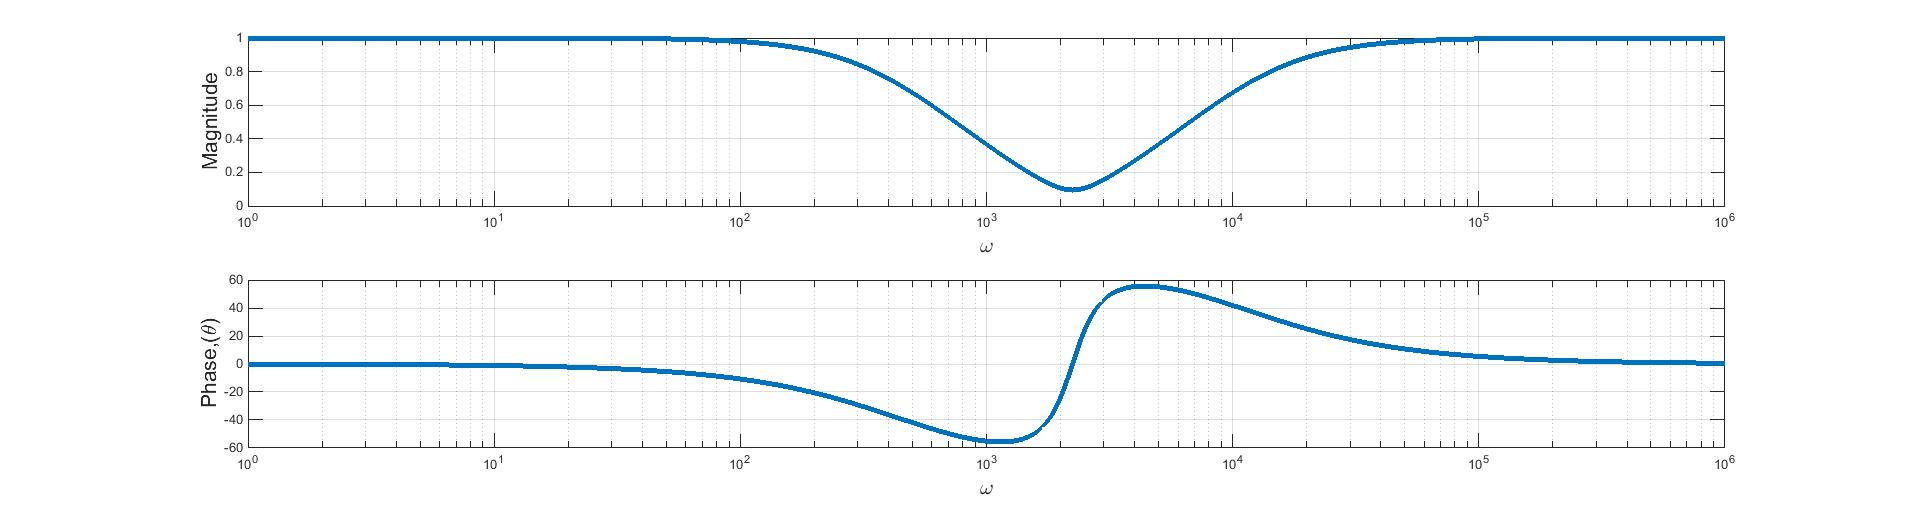
\includegraphics[width=1\textwidth]{Example2soln.jpg}
\end{figure}

The magnitude response is what we would expect for a BRF and the phase response is zero in both passbands.
}

\newpage
\clearpage
\pagebreak

\textbf{How do we build this filter?}
To start, let's look once again at the block diagram of the BRF:
\begin{figure} [h!]
\centering
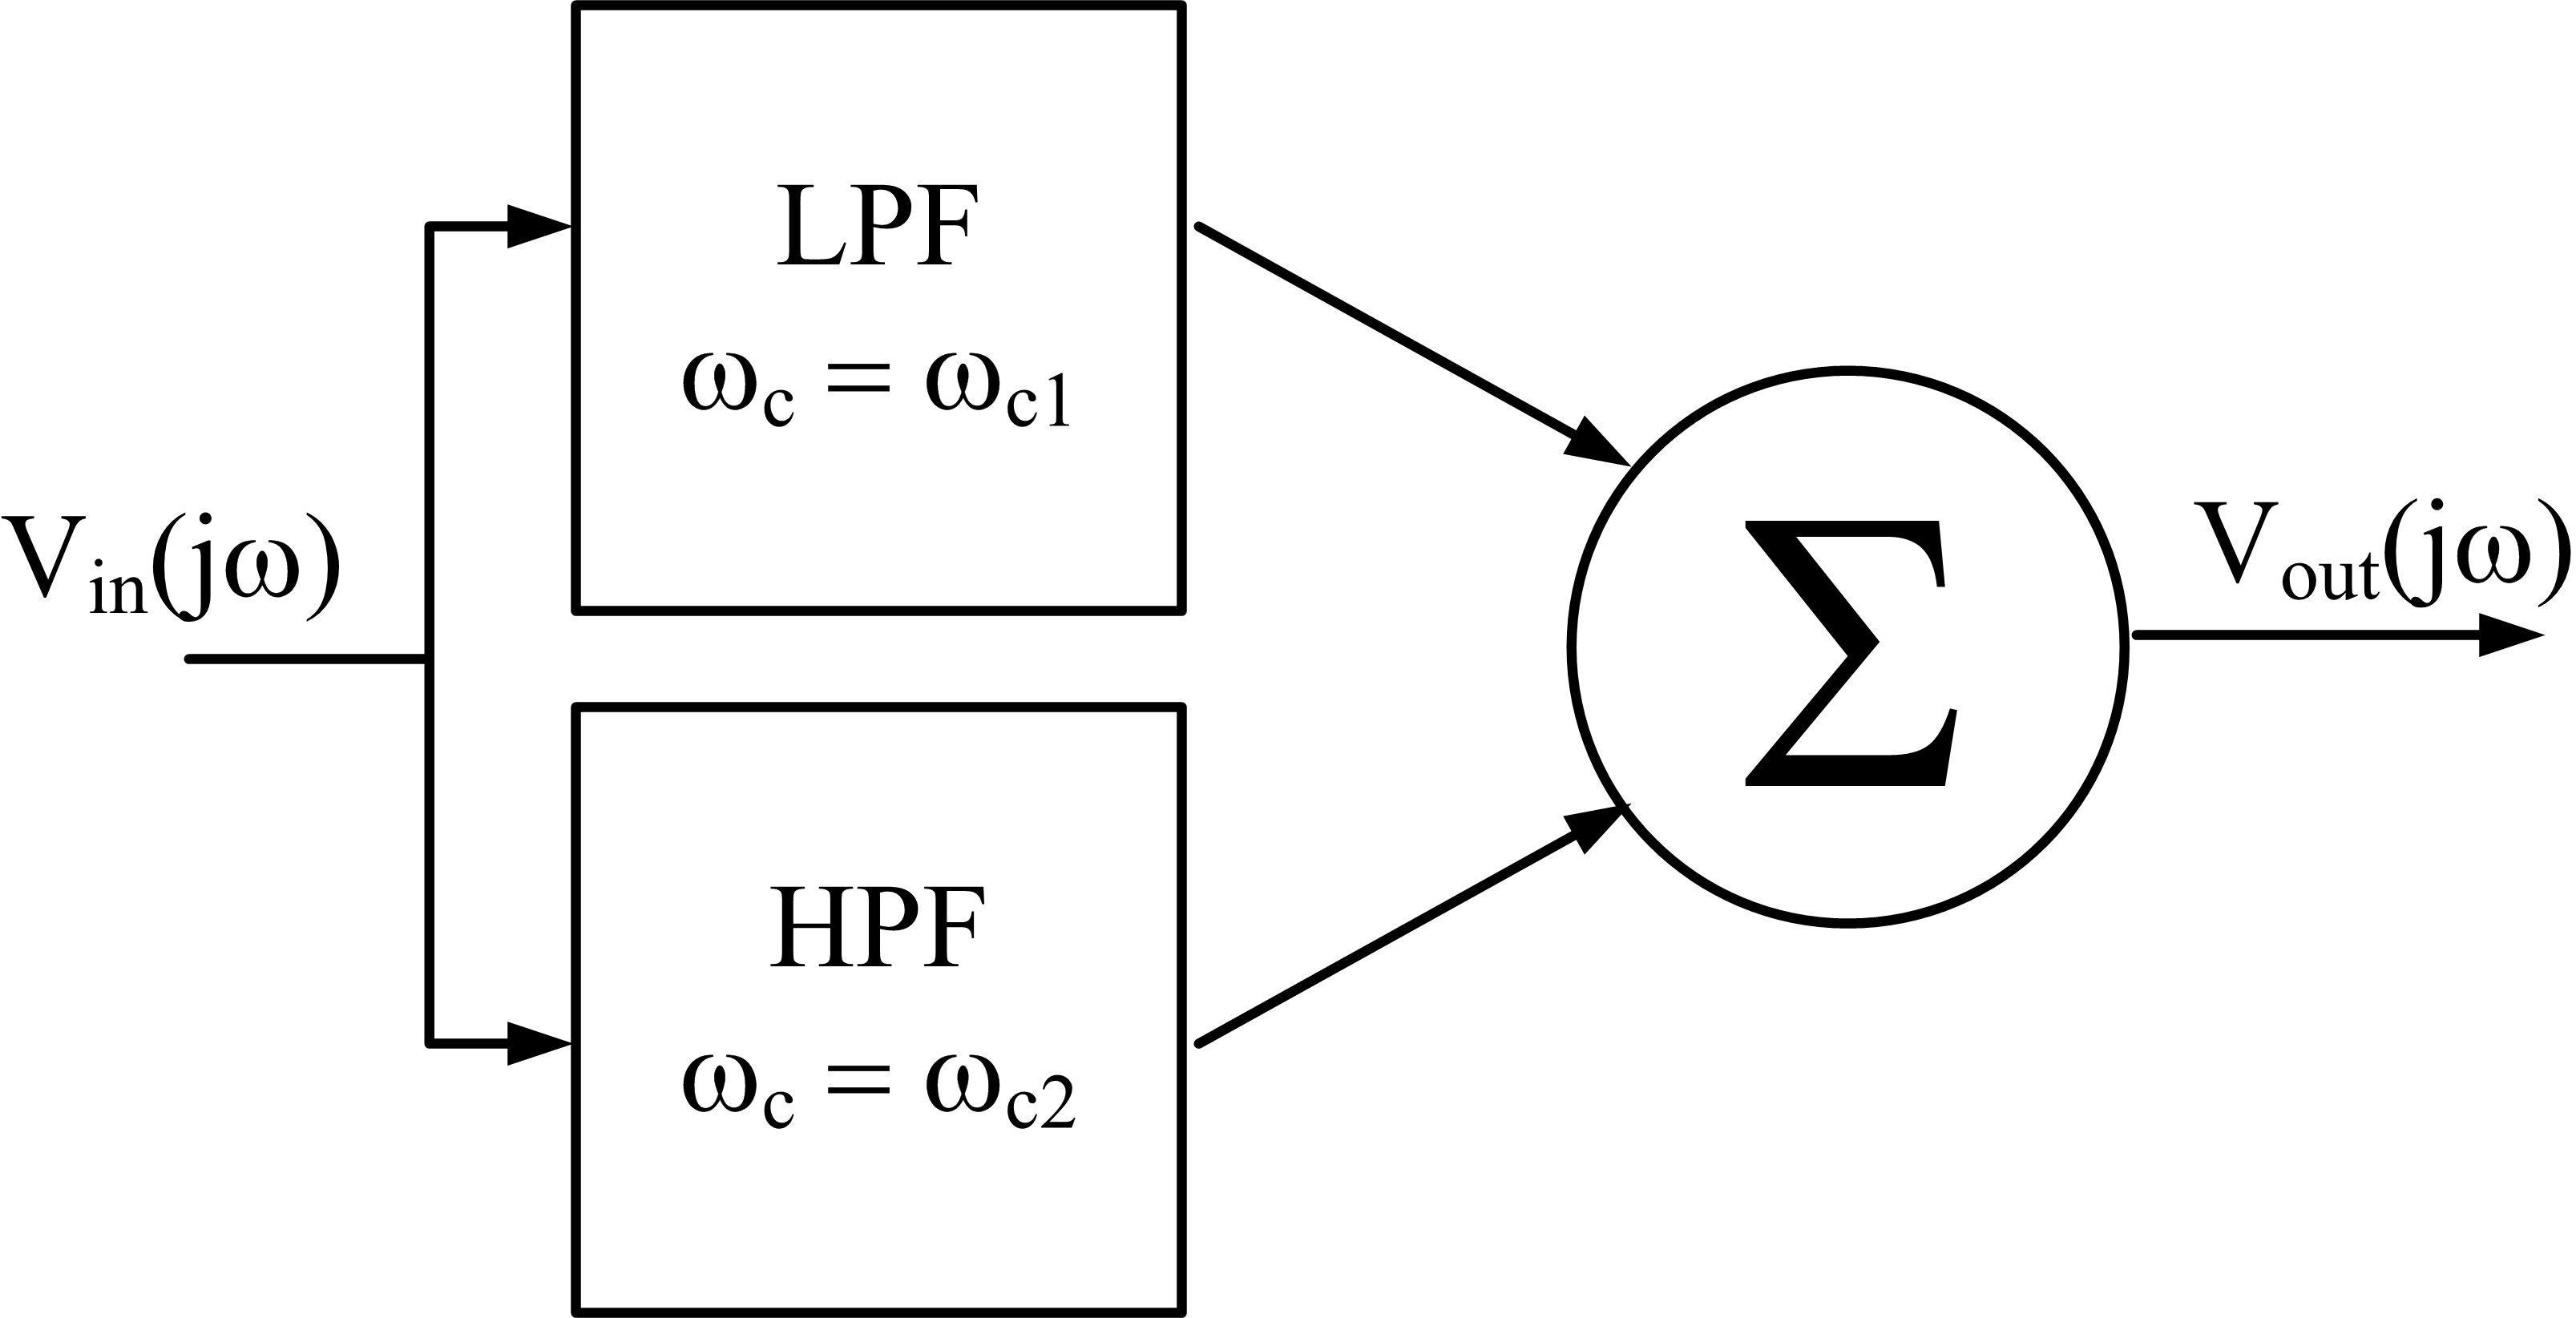
\includegraphics[width=0.5\textwidth]{BRFBlockDiagram.jpg}
\end{figure}

By looking at this figure, it should be clear that we will need a HPF, a LPF and a summer (remember that thing we built with op amps); what might not be obivous yet is that we will also need a couple of buffers.

Let's jump into the design:

\soln{8in}{
Let's start with our LPF design; from our standard form of a LPF transfer function, we know:
\[
\frac{1}{R_{LPF}C_{LPF}}=500\frac{rad}{s}
\]
so let's use
\[
R_{LPF} = 20\ k\Omega
\]
\[
C_{LPF}=0.1\ \mu F
\]

Next we move to the HPF design.  Again from our standard form for a HPF transfer function we can know:
\[
\frac{1}{R_{HPF}C_{HPF}}=10,000\frac{rad}{s}
\]
so let's use
\[
R_{HPF} = 1\ k\Omega
\]
\[
C_{HPF}=0.1\ \mu F
\]
}

\newpage
\clearpage
\pagebreak

We now tie the filters together using a summer (\textbf{DO NOT JUST TIE THE OUTPUTS TOGETHER!})

\soln{8in}{
This figure is hidden is student copy
\begin{figure} [h!]
\centering
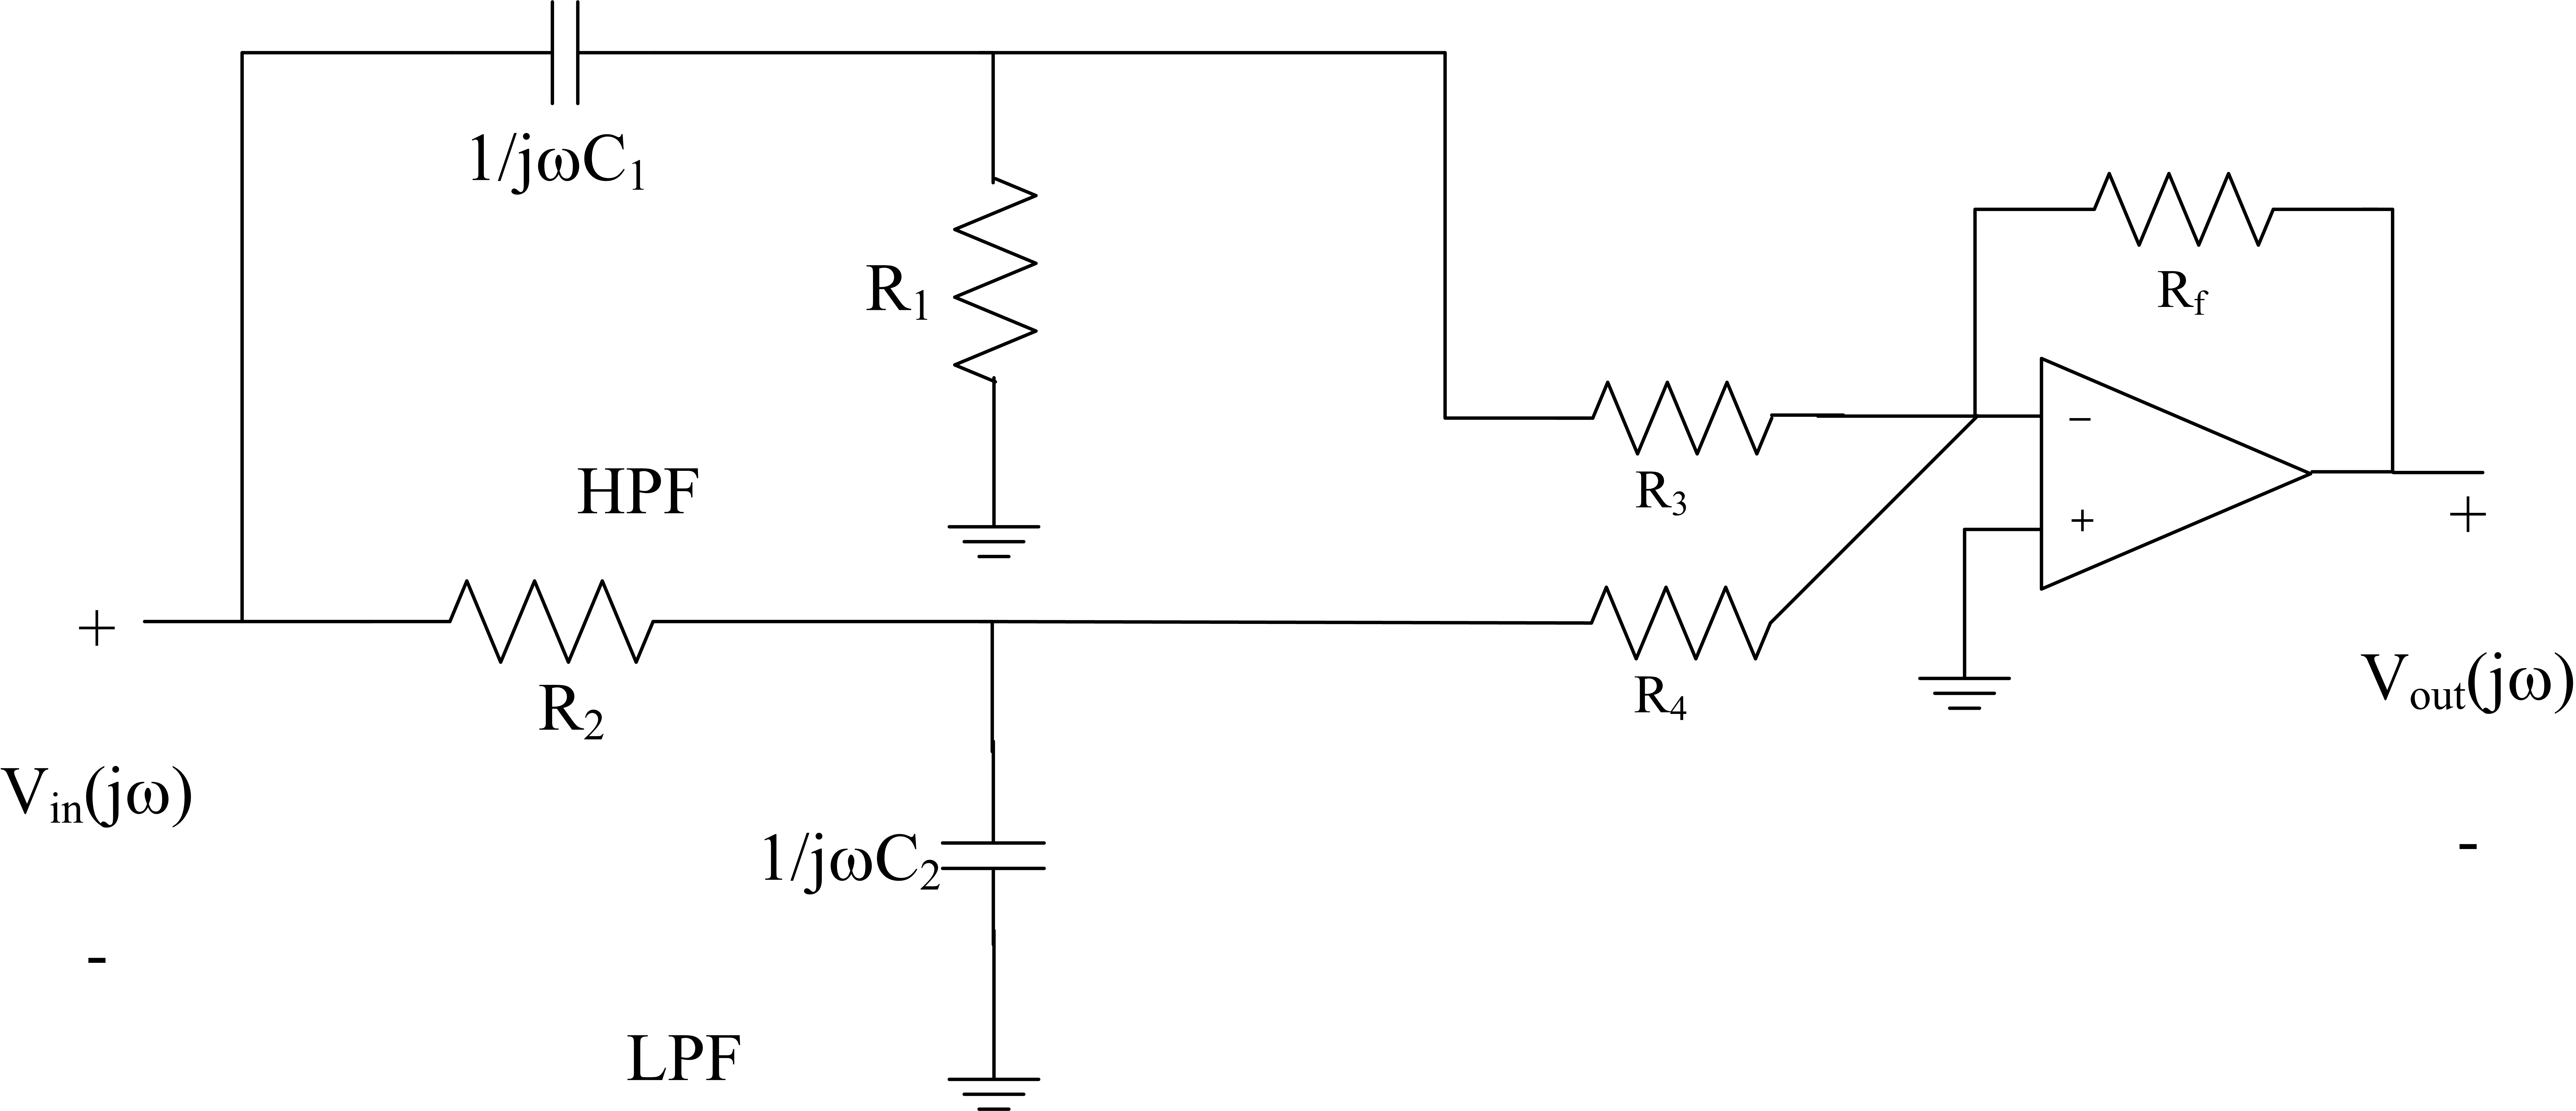
\includegraphics[width=0.8\textwidth]{BRF1.jpg}
\end{figure}

In this and the next figure $C_1=C_{HPF}$, $R_1 = R_{HPF}$, $C_2=C_{LPF}$, and $R_2=R_{LPF}$

But there is a problem here.... We know an inverting summer can suffer from input loading.  We need to put buffers on the summer inputs:

This figure is hidden is student copy
\begin{figure} [h!]
\centering
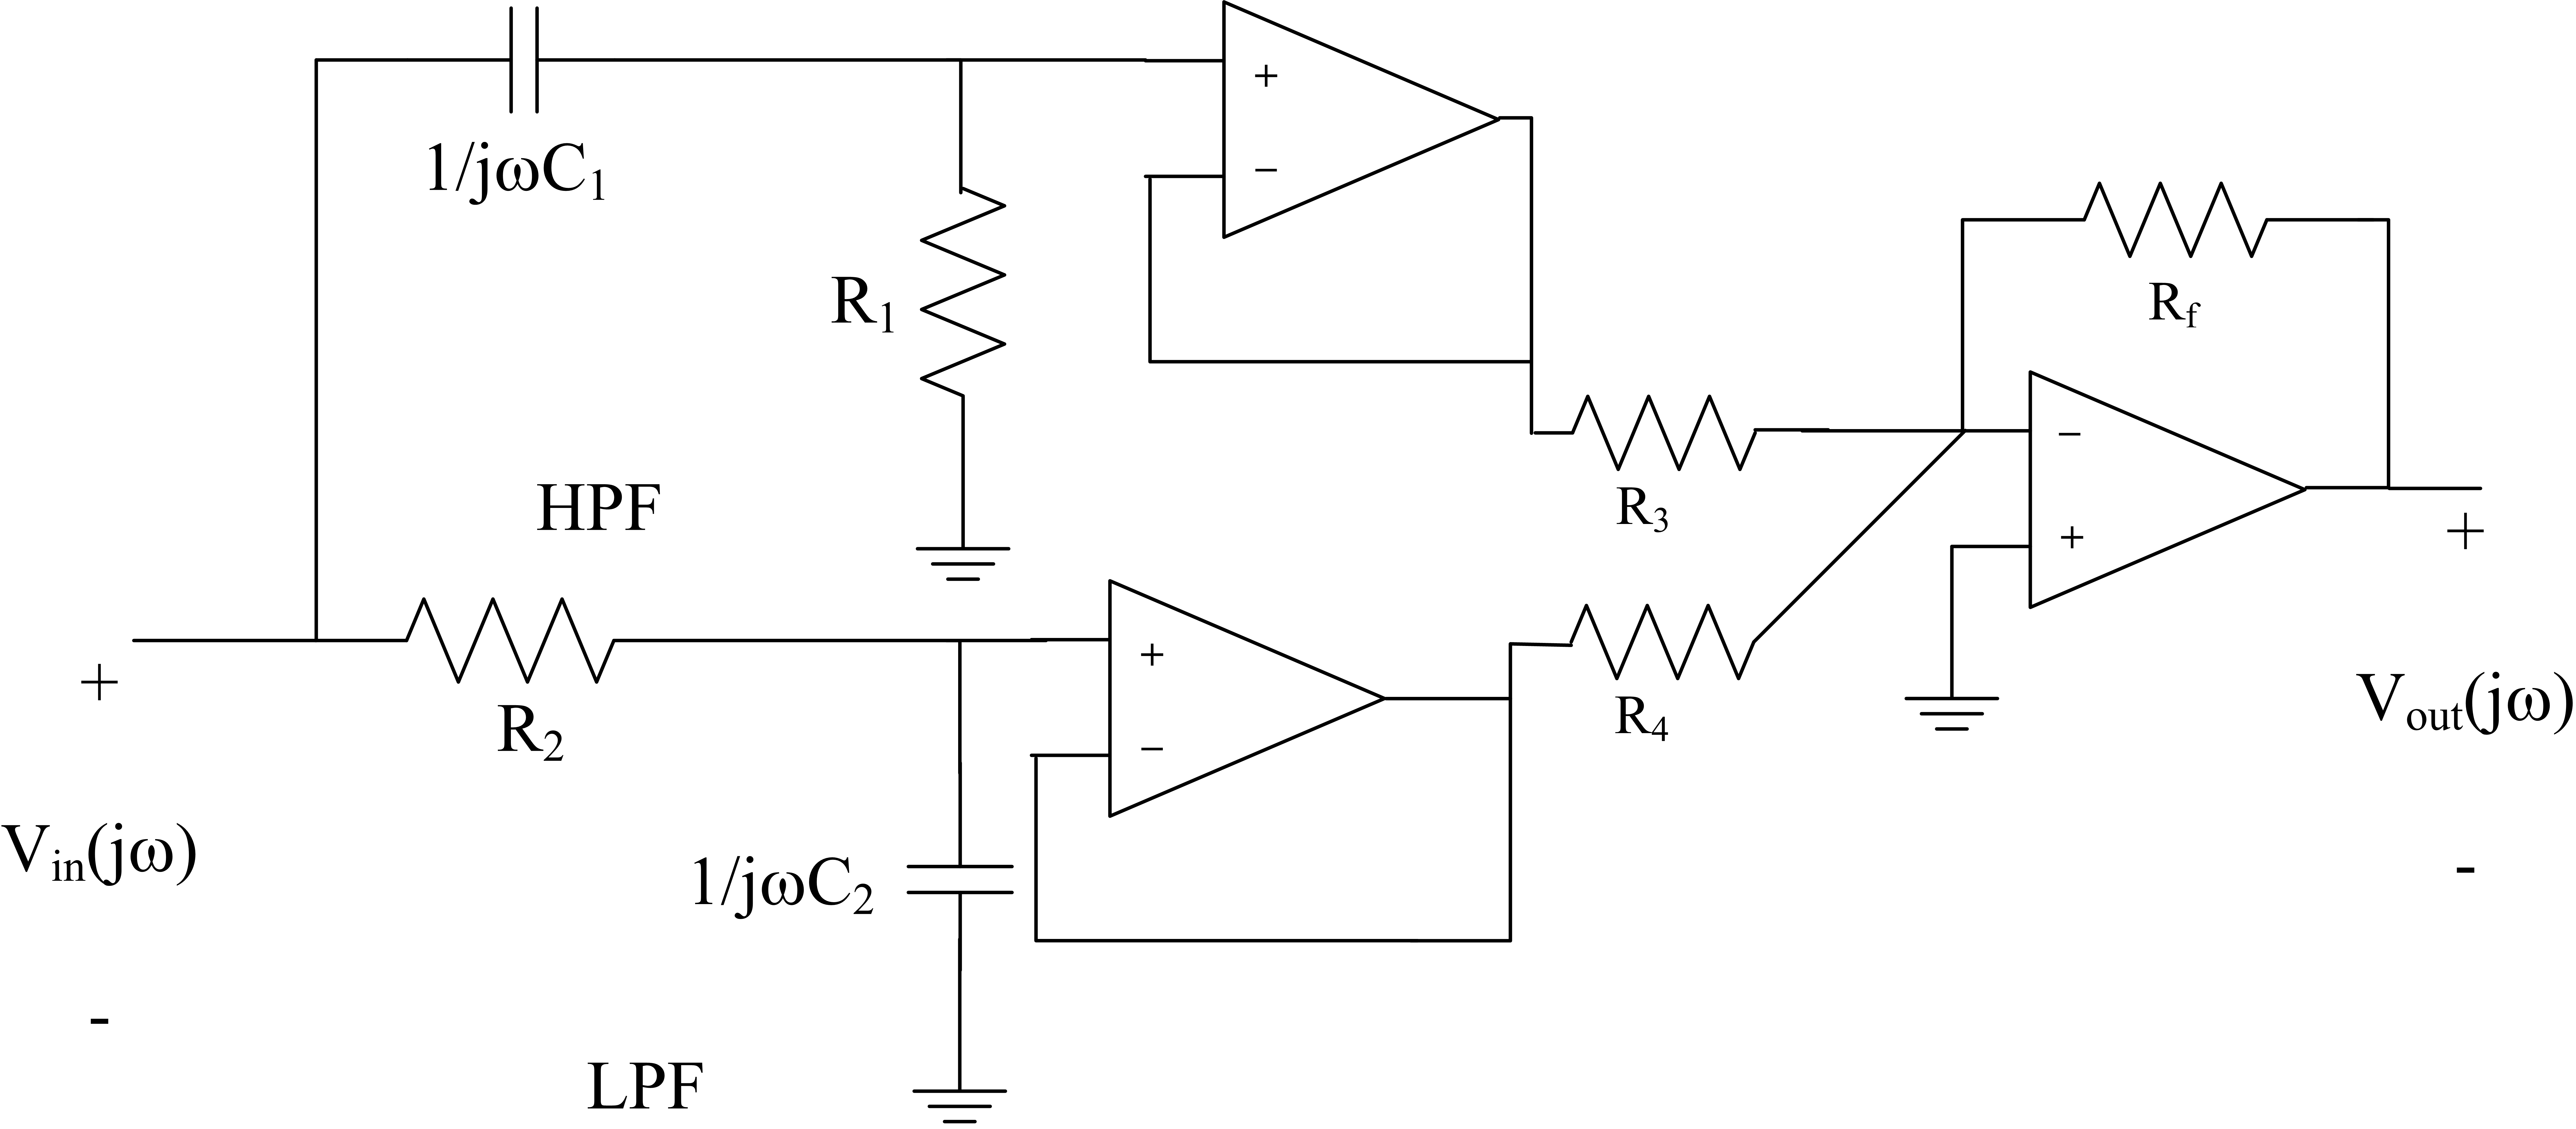
\includegraphics[width=0.8\textwidth]{BRF2.jpg}
\end{figure}
}

This filter design would give us the magnitude and phase response we expect from a BRF, with one exception.  The inverting nature of the summer would cause a $180^o$ phase shift in the output.


\newpage
\clearpage
\pagebreak

\end{document}


% Equation Array Example Code
%\begin
%{eqnarray}
%P_R &=& i_R^2R \nonumber \\
%P_R &=& (100\ mA)^2 \times 100\ \Omega \nonumber \\
%P_R &=& (100 \times 10^{-3}\ A)^2 \times 100\ \Omega \\
%P_R &=& 10000 \times 10^{-6}\ A^2  \times 100\ \Omega \nonumber \\
%P_R &=& 1\ W  \nonumber
%\end{eqnarray}

% Figure Example Code
%\begin{figure} [h!]
%\centering
%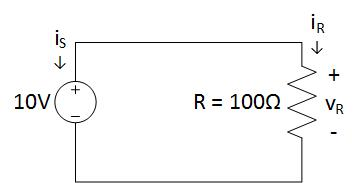
\includegraphics[width=0.5\textwidth]{OhmsLawExampleSolution.jpg}
%\caption{Ohm's Law example circuit}
%\label{fig: OhmsLawExampleSolution}
%\end{figure}

%Table Example Code
%\begin{table}[h]
%\centering
%\begin{tabular}{|l|c|c|}
%\hline
%Prefix & Abbreviation & Value \\
%\hline \hline
%Giga & $G$ & $10^9$ \\
%Mega & $M$ & $10^6$ \\
%Kilo & $k$ & $10^3$ \\
%\hline
%milli & $m$ & $10^{-3}$ \\
%micro & $\mu$ & $10^{-6}$ \\
%nano & $n$ & $10^{-9}$ \\
%pico & $p$ & $10^{-12}$ \\
%\hline
%\end{tabular}
%\caption{Engineering prefixes and values}
%\label{tab: Eng Prefixes}
%\end{table}
